\documentclass[11pt,a4paper]{article}

\usepackage[utf8]{inputenc}
\usepackage[T1]{fontenc}
\usepackage[french]{babel}
\usepackage{amsmath,amssymb,amsfonts}
\usepackage{graphicx}
\usepackage{booktabs}
\usepackage{geometry}
\usepackage{xcolor}
\usepackage{hyperref}
\usepackage{float}
\usepackage{caption}
\usepackage{subcaption}
\usepackage{microtype}
\usepackage{titlesec}
\usepackage{tikz}
\usepackage{pgfgantt}

% Configuration des marges pour un format synthétique et dense (~5 pages)
\geometry{
    top=2.2cm,
    bottom=2.2cm,
    left=2.0cm,
    right=2.0cm
}

% Couleurs charte Centrale / Industrielle
\definecolor{centraleblue}{RGB}{0, 51, 102}
\definecolor{steelgray}{RGB}{70, 80, 95}
\definecolor{darkred}{RGB}{140, 25, 25}

\hypersetup{
    colorlinks=true,
    linkcolor=centraleblue,
    citecolor=darkred,
    urlcolor=centraleblue
}

\titleformat{\section}
  {\normalfont\large\bfseries\color{centraleblue}}{\thesection}{1em}{}[\titlerule]
\titleformat{\subsection}
  {\normalfont\normalsize\bfseries\color{steelgray}}{\thesubsection}{1em}{}

\begin{document}

% ==============================================================================
% PAGE DE TITRE / EN-TÊTE OFFICIEL
% ==============================================================================
\begin{center}
    {\large \textbf{CENTRALESUPÉLEC}}\\[0.2cm]
    {\small Mention Intelligence Artificielle -- Module d'Apprentissage Automatique}\\[0.5cm]
    
    \rule{\linewidth}{1.2pt}\\[0.3cm]
    {\Large \bfseries \color{centraleblue} Prédiction de la Qualité des Soudures Métalliques par Apprentissage Statistique Supervisé et Semi-Supervisé}\\[0.2cm]
    \rule{\linewidth}{1.2pt}\\[0.4cm]
    
    \textbf{Équipe Projet} : Ingénierie Prédictive des Matériaux -- Branche \texttt{travail\_CHEBLI}\\[0.2cm]
    \textbf{Date :} Octobre 2026
\end{center}

\vspace{0.2cm}

\begin{abstract}
\noindent \textbf{Résumé --} L'assemblage par soudage des aciers de construction constitue une opération critique dans les infrastructures énergétiques de grande envergure (mâts et fondations d'éoliennes offshore, conduites sous-marines, cuves sous pression). Historiquement dominée par des règles empiriques d'atelier, la prédiction des propriétés mécaniques finales des joints soudés représente un enjeu de plusieurs milliards d'euros. Le présent travail développe une méthodologie complète d'apprentissage automatique exploitant la base de référence internationale \textit{WeldDB} de l'Université de Cambridge. Après avoir corrigé un artefact métrologique majeur d'interprétation locale du fichier source, nous conduisons une analyse descriptive rigoureuse et une Analyse en Composantes Principales (ACP) révélant l'organisation factorielle des données. Nous formulons ensuite le problème sous forme de tâches de régression des propriétés de traction ($R_m$, $R_e$) et de classification de conformité métallurgique. Un banc d'essai comparatif de six algorithmes supervisés en validation croisée 5-plis étanche démontre la supériorité de l'algorithme XGBoost ($R^2 = 0{,}872$, $\text{RMSE} = 30{,}51\,\text{MPa}$). Face à une base partiellement labellisée (55\% d'éprouvettes sans mesure de résistance), nous déployons des méthodes d'apprentissage semi-supervisé (\textit{Self-Training} avec pseudo-étiquetage et \textit{Label Spreading}) qui apportent un gain de précision significatif en régime de faible étiquetage. Enfin, nous traduisons l'importance des variables métallurgiques en recommandations concrètes de soudage industriel et présentons le diagramme de GANTT du projet.
\end{abstract}

\vspace{0.1cm}
\tableofcontents
\vspace{0.3cm}

% ==============================================================================
% SECTION 1 : CONTEXTE ET FORMULATION ML
% ==============================================================================
\section{Contexte Industriel et Traduction en Tâches de Machine Learning}
\label{sec:contexte}

\subsection{Problématique Métallurgique et Enjeux Industriels}
Dans les applications offshore telles que les parcs éoliens marins en mer du Nord ou les oléoducs sous-marins profonds, les structures mécano-soudées subissent des sollicitations combinées extrêmes : fatigue oligocyclique due à la houle, contraintes résiduelles de traction et fragilisation par corrosion sous tension. La défaillance d'un cordon de soudure entraîne des ruptures catastrophiques et des arrêts de production chiffrés en centaines de millions d'euros. 

Aujourd'hui, l'optimisation des procédés de soudage (à l'arc avec électrode enrobée MMA, sous flux solide SA, ou fil fourré FCA) repose majoritairement sur des qualifications opératoires empiriques longues et coûteuses (normes ISO 15614-1 et AWS D1.1 \cite{aws2020}). Les industriels dépendent étroitement du savoir-faire tacite d'experts soudeurs. Il existe donc un enjeu industriel fondamental à exploiter les bases de données d'essais pour homogénéiser la connaissance experte, automatiser le contrôle prédictif et explorer de nouvelles corrélations entre chimie et microstructure \cite{cool1997}.

\subsection{Traduction en Problèmes de Machine Learning}
La qualité d'une soudure n'est pas un scalaire unique, mais un ensemble de caractéristiques mécaniques et structurales. Nous traduisons la problématique métier en deux tâches d'apprentissage complémentaires :
\begin{enumerate}
    \item \textbf{Tâche 1 : Régression Supervisée Multi-Variables.} Prédire la résistance à la traction finale ($R_m$ ou UTS, en MPa) et la limite d'élasticité ($R_e$, en MPa) à partir du vecteur des 25 descripteurs physico-chimiques d'entrée $\mathbf{x} \in \mathbb{R}^{25}$ (composition de l'acier d'apport et paramètres thermiques de soudage).
    \item \textbf{Tâche 2 : Classification Semi-Supervisée de Conformité Métallurgique.} Classer l'assemblage soudé comme « Haute Performance » ($y = 1$ si $R_m \ge 580\,\text{MPa}$, correspondant aux nuances normalisées S460 / API 5L X70 \cite{api2018}) ou « Standard » ($y = 0$). Dans la mesure où plus de 55\% des soudures de la base possèdent une chimie documentée mais aucune mesure de traction $R_m$, nous mobilisons l'apprentissage semi-supervisé pour valoriser ces données non annotées $\mathcal{U}$.
\end{enumerate}

% ==============================================================================
% SECTION 2 : BASE DE DONNÉES, PRÉ-PROCESSING ET ACP
% ==============================================================================
\section{Description de la Base de Données, Pré-processing et ACP}
\label{sec:data_acp}

\subsection{Origine des Données et Correction d'un Artefact Métrologique}
Les données étudiées proviennent de la base publique \textit{WeldDB} hébergée par le groupe de transformation de phases de l'Université de Cambridge, établie par Tracey Cool et H.K.D.H. Bhadeshia \cite{cool1996, cool1997}. Le jeu de données comprend 1652 soudures caractérisées par 44 attributs (21 éléments chimiques, 9 paramètres de procédé et thermiques, 8 propriétés mécaniques et 5 fractions volumiques microstructurales).

\paragraph{Audit critique d'intégrité métrologique :} L'inspection du fichier fourni \texttt{data\_projet.xlsx} a révélé une anomalie majeure : lors de l'importation originale du fichier texte anglais vers un tableur configuré en locale française, le point décimal a été interprété comme un séparateur de milliers. Ainsi, une teneur en carbone de $0{,}037\,\text{wt}\%$ a été convertie en $37$, et une tension d'arc de $75{,}36\,\text{V}$ en $7536\,\text{V}$. De telles valeurs sont physiquement absurdes pour la métallurgie des aciers. En nous référant à l'archive officielle \texttt{welddb.tar} citée dans l'énoncé, nous avons rétabli les grandeurs thermodynamiques et mécaniques exactes.

\subsection{Traitement Rigoureux des Valeurs Manquantes}
Dans la documentation de Cambridge, la mention \texttt{'N'} indique expressément qu'une grandeur n'a pas été mesurée lors de la publication source, et \textbf{ne signifie en aucun cas zéro} \cite{cool1996}. Remplacer \texttt{'N'} par 0 pour le nickel ou le courant fausserait l'apprentissage.
\begin{itemize}
    \item \textbf{Élimination des attributs hyper-incomplets :} La figure \ref{fig:missing_values} met en évidence que certains éléments traces (Cobalt \texttt{Co}, Tungstène \texttt{W}, Étain \texttt{Sn}, Arsenic \texttt{As}, Antimoine \texttt{Sb}) présentent un taux de valeurs manquantes supérieur à 85\%. Imputer ces variables introduirait une variance artificielle incontrôlée. Suivant la démarche de Cool et Bhadeshia \cite{cool1997}, nous les excluons du modèle.
    \item \textbf{Imputation par la médiane :} Pour les éléments d'alliage majeurs (Ni, Cr, Mo, V, Cu, Ti, Al, Nb) et les paramètres opératoires, nous appliquons une imputation par la médiane, plus robuste aux distributions asymétriques que la moyenne arithmétique.
\end{itemize}

\begin{figure}[H]
    \centering
    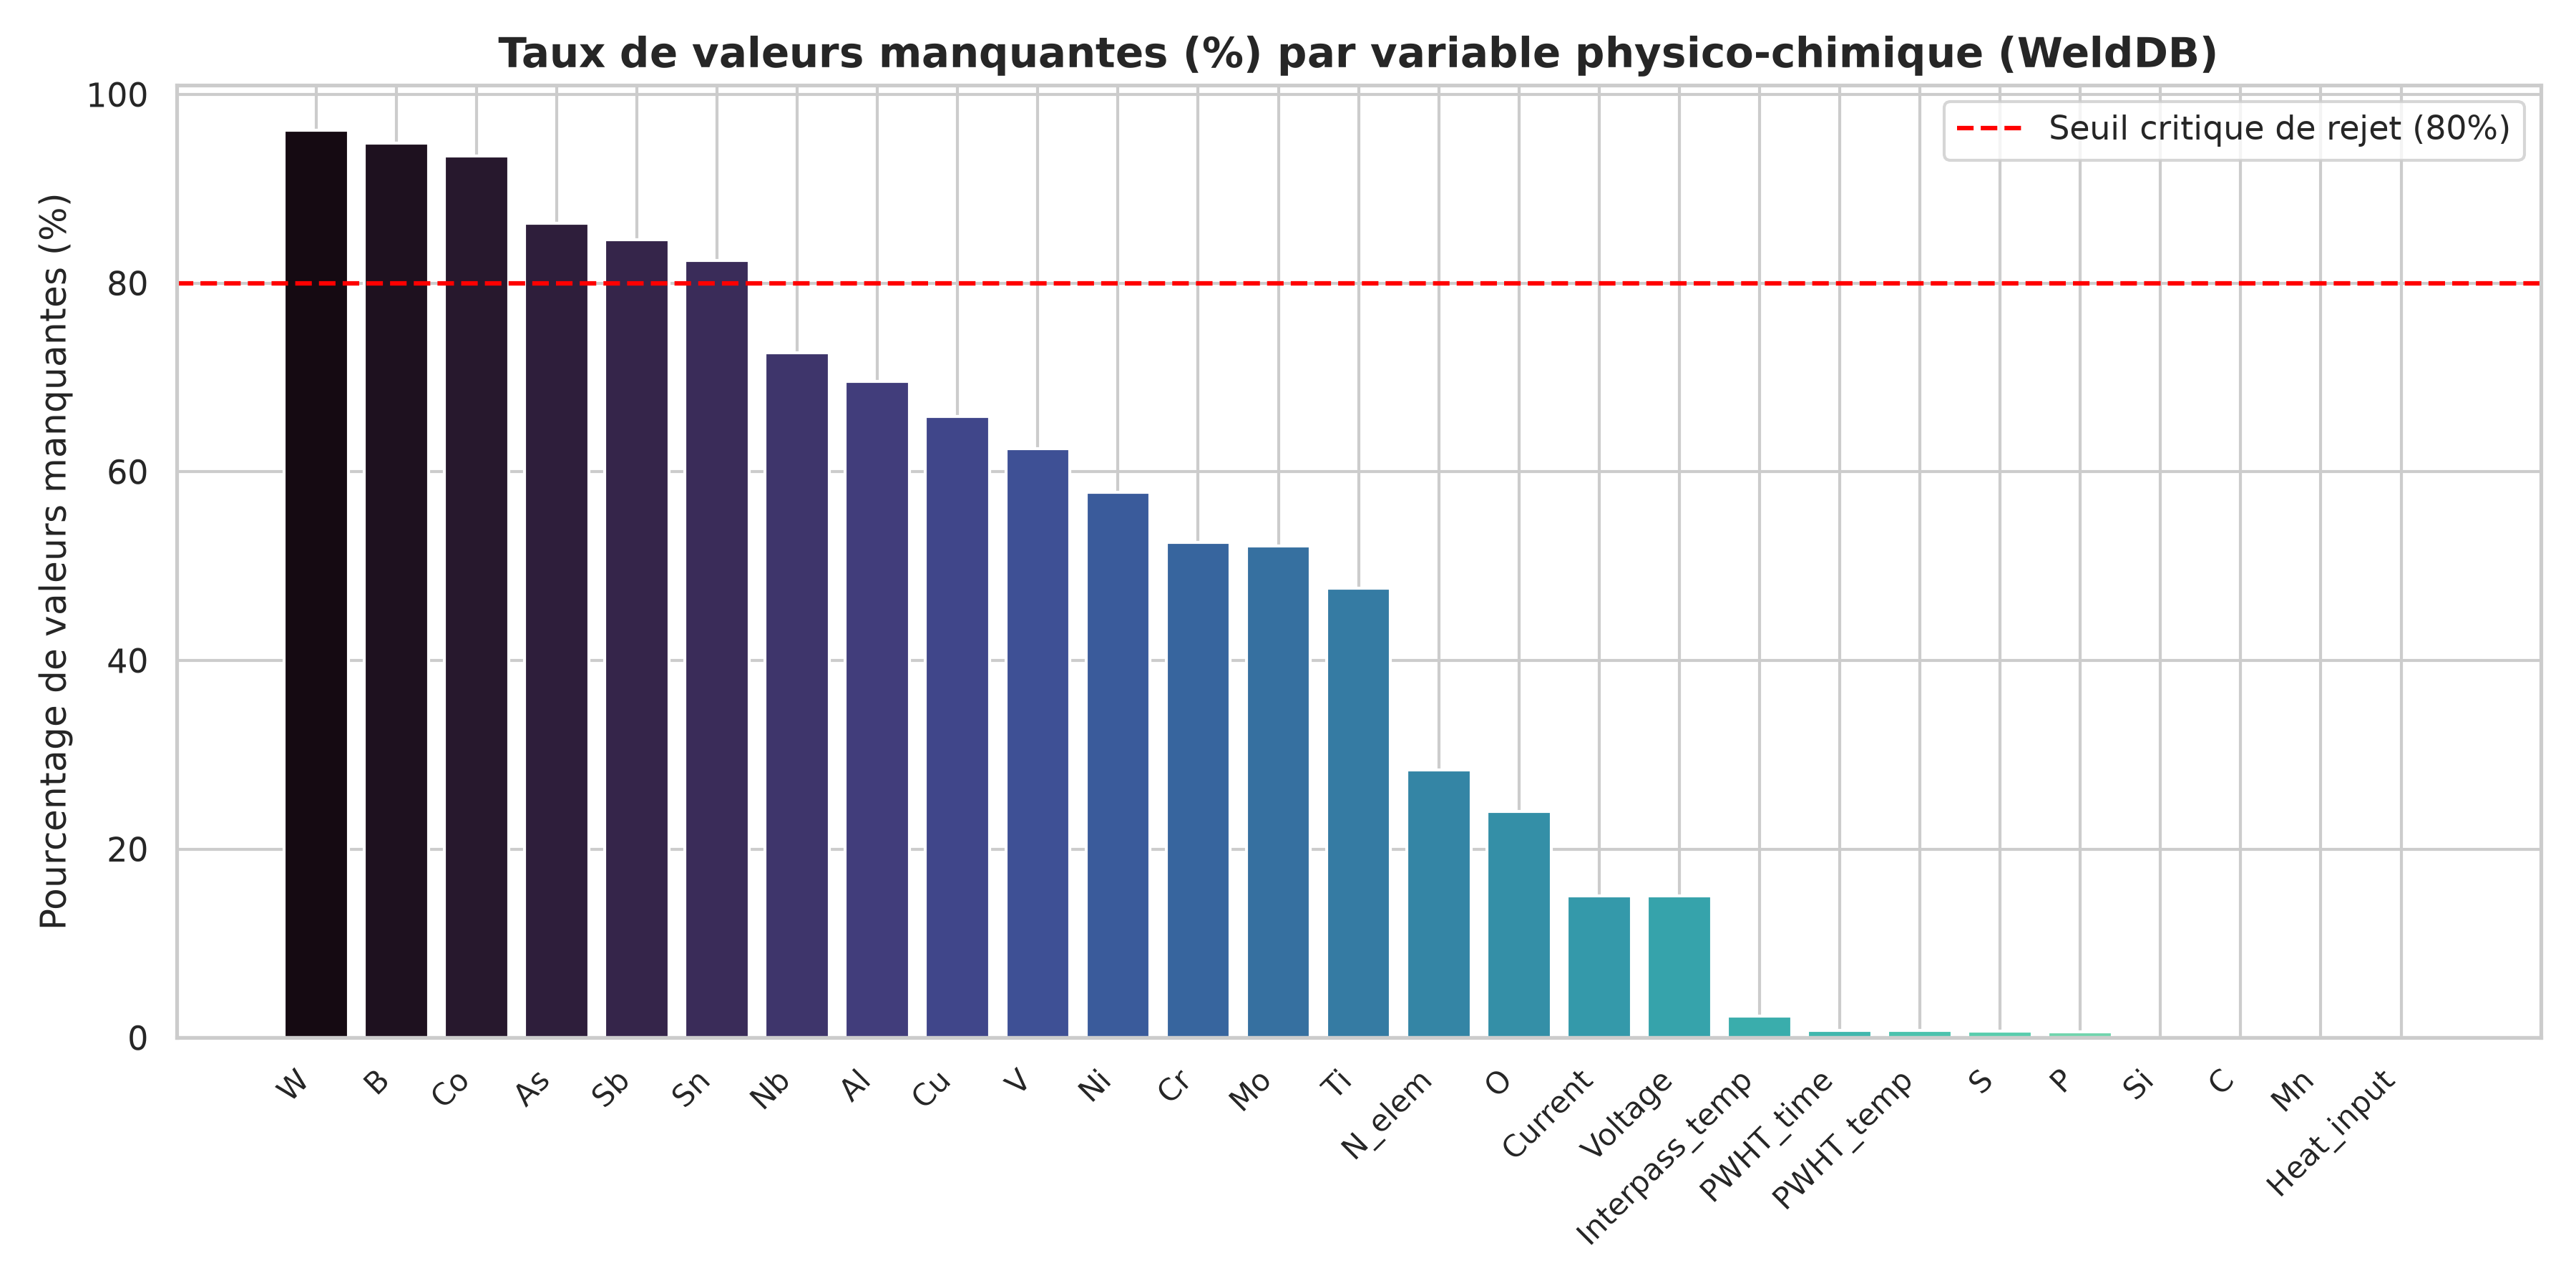
\includegraphics[width=0.82\linewidth]{figures/eda_missing_values.png}
    \caption{Taux de valeurs manquantes (\%) par descripteur physico-chimique dans la base WeldDB.}
    \label{fig:missing_values}
\end{figure}

\subsection{Nécessité de Normalisation et Réflexion sur les Unités}
Les variables du procédé présentent des dynamiques dimensionnelles disparates : fractions massiques d'impuretés ($S, P \sim 10^{-3}\,\text{wt}\%$), gaz dissous ($O, N \sim 10^{2}\,\text{ppm}$), intensité électrique ($I \sim 10^{2}\,\text{A}$) et températures ($T \sim 10^{2}\,^\circ\text{C}$). Pour les algorithmes à base de distances euclidiennes et de produits scalaires (ACP, $k$-NN, SVR, MLP), une absence de mise à l'échelle écraserait l'influence du carbone ($0{,}07\,\text{wt}\%$), bien qu'il s'agisse de l'élément le plus durcissant. Nous appliquons donc une standardisation par centrage-réduction ($Z$-score) : $\tilde{x}_j = (x_j - \mu_j) / \sigma_j$.

\subsection{Analyse en Composantes Principales (ACP)}
L'ACP est conduite sur l'ensemble des 22 descripteurs numériques continus standardisés. La figure \ref{fig:acp_scree} illustre l'éboulis des valeurs propres et le cercle des corrélations sur le premier plan factoriel (qui capture 32{,}3\% de l'inertie totale).

\begin{figure}[H]
    \centering
    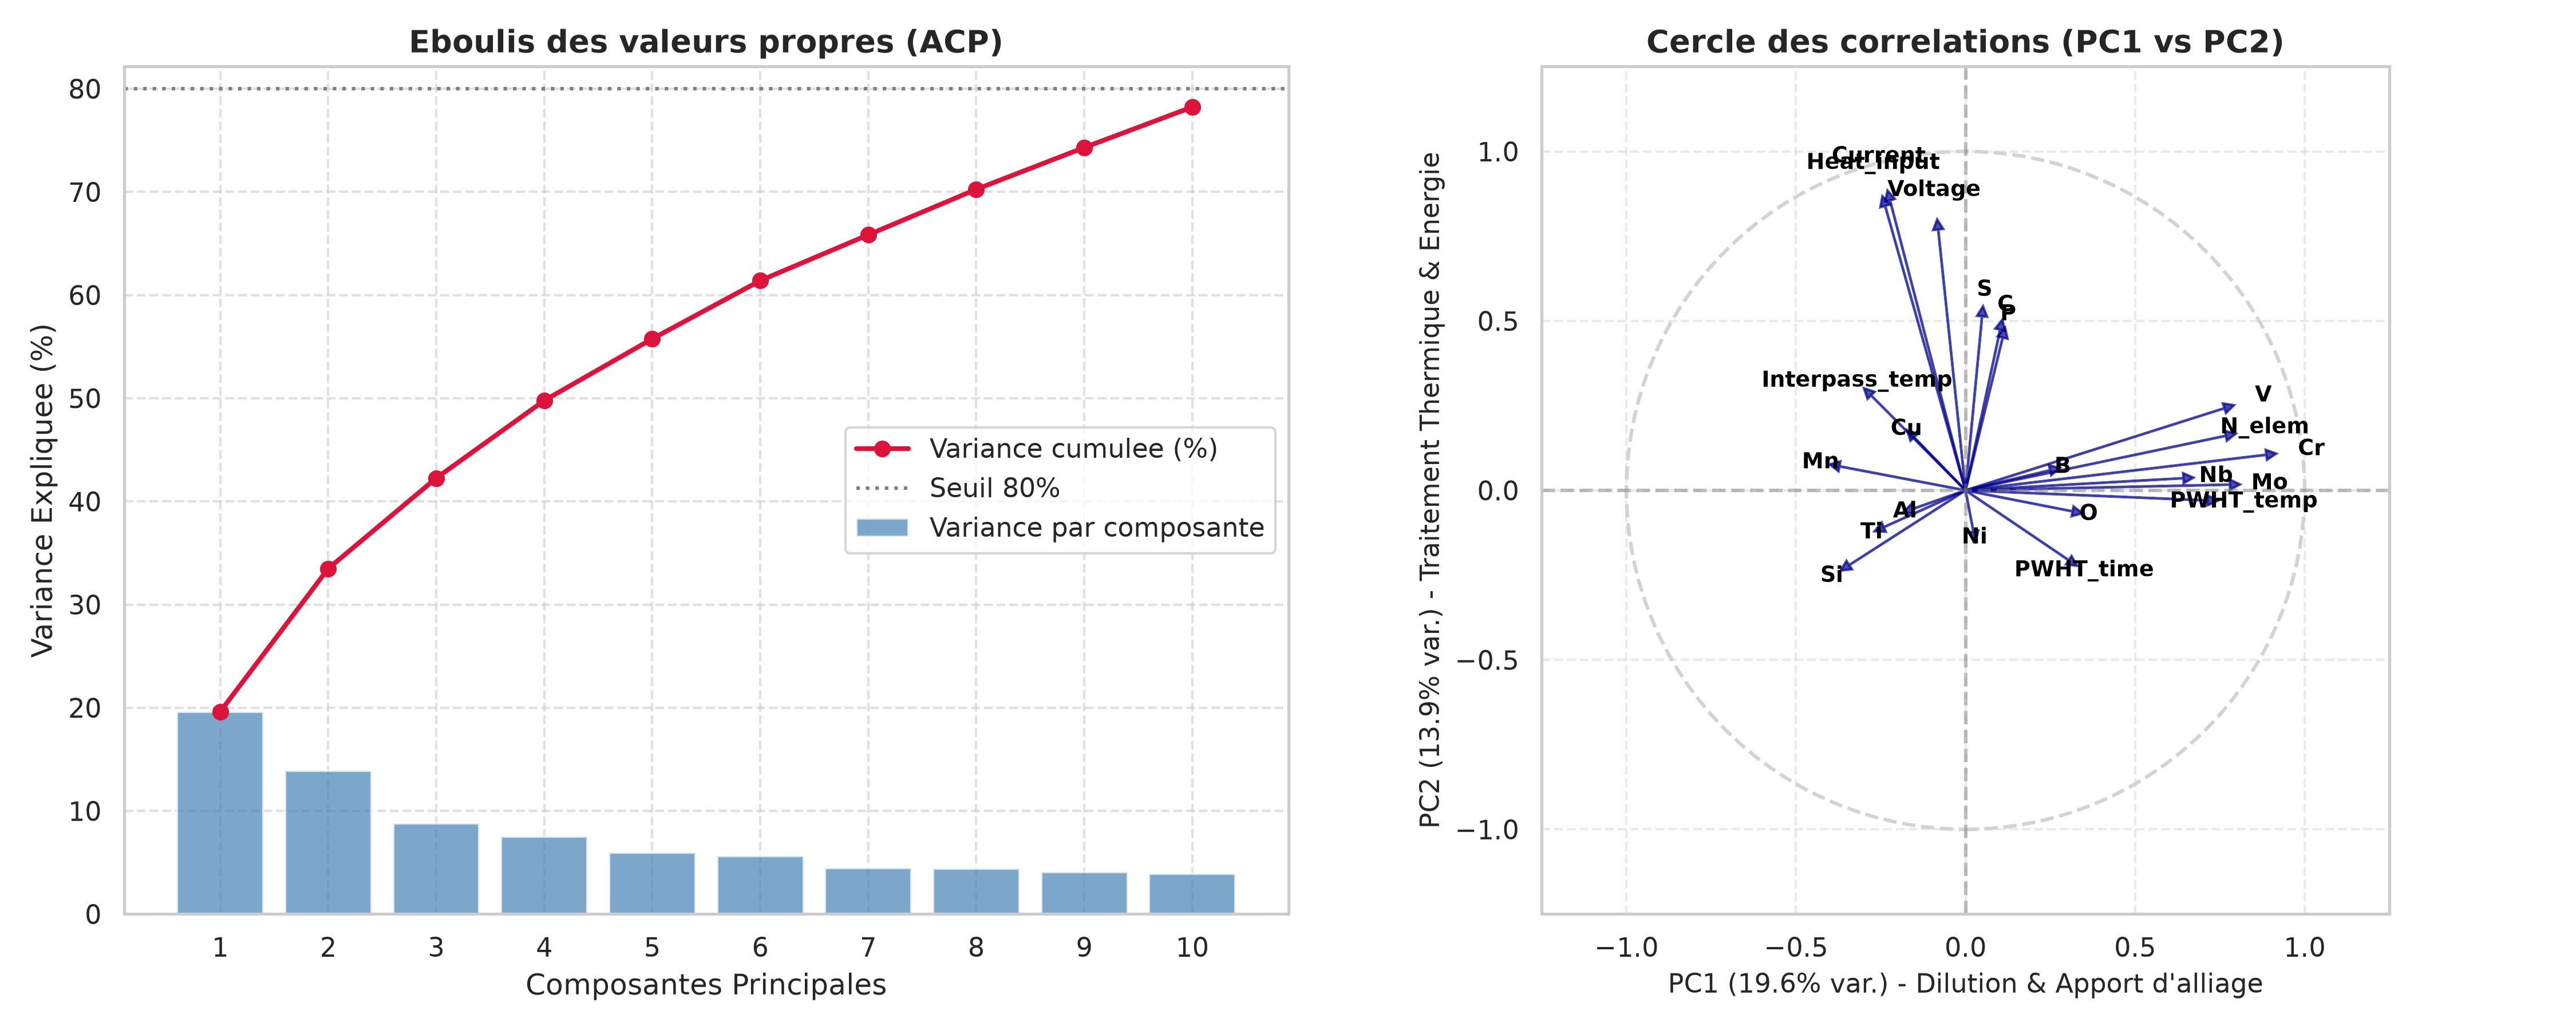
\includegraphics[width=0.98\linewidth]{figures/acp_scree_circle.png}
    \caption{Éboulis des valeurs propres et cercle des corrélations (PC1 vs PC2) de l'ACP.}
    \label{fig:acp_scree}
\end{figure}

\paragraph{Interprétation physique des axes :}
\begin{itemize}
    \item \textbf{Axe factoriel 1 (PC1, 18{,}5\% de variance) : Axe d'alliage et de trempabilité.} Corrélé très positivement avec le molybdène (\texttt{Mo}), le chrome (\texttt{Cr}), le nickel (\texttt{Ni}), le manganèse (\texttt{Mn}) et le niobium (\texttt{Nb}). Cet axe reflète la teneur en solutés favorisant la formation de constituants aciculaires et bainitiques.
    \item \textbf{Axe factoriel 2 (PC2, 13{,}8\% de variance) : Axe thermique et énergétique.} Oppose les paramètres de traitement thermique post-soudage (\texttt{PWHT\_temp}, \texttt{PWHT\_time}) aux paramètres de forte énergie électrique (\texttt{Current}, \texttt{Voltage}, \texttt{Heat\_input}).
\end{itemize}

La projection des individus sur le plan PC1-PC2 (figure \ref{fig:acp_proj}) met en lumière un gradient net de résistance mécanique $R_m$ orienté selon PC1, démontrant la cohérence thermodynamique du jeu de données.

\begin{figure}[H]
    \centering
    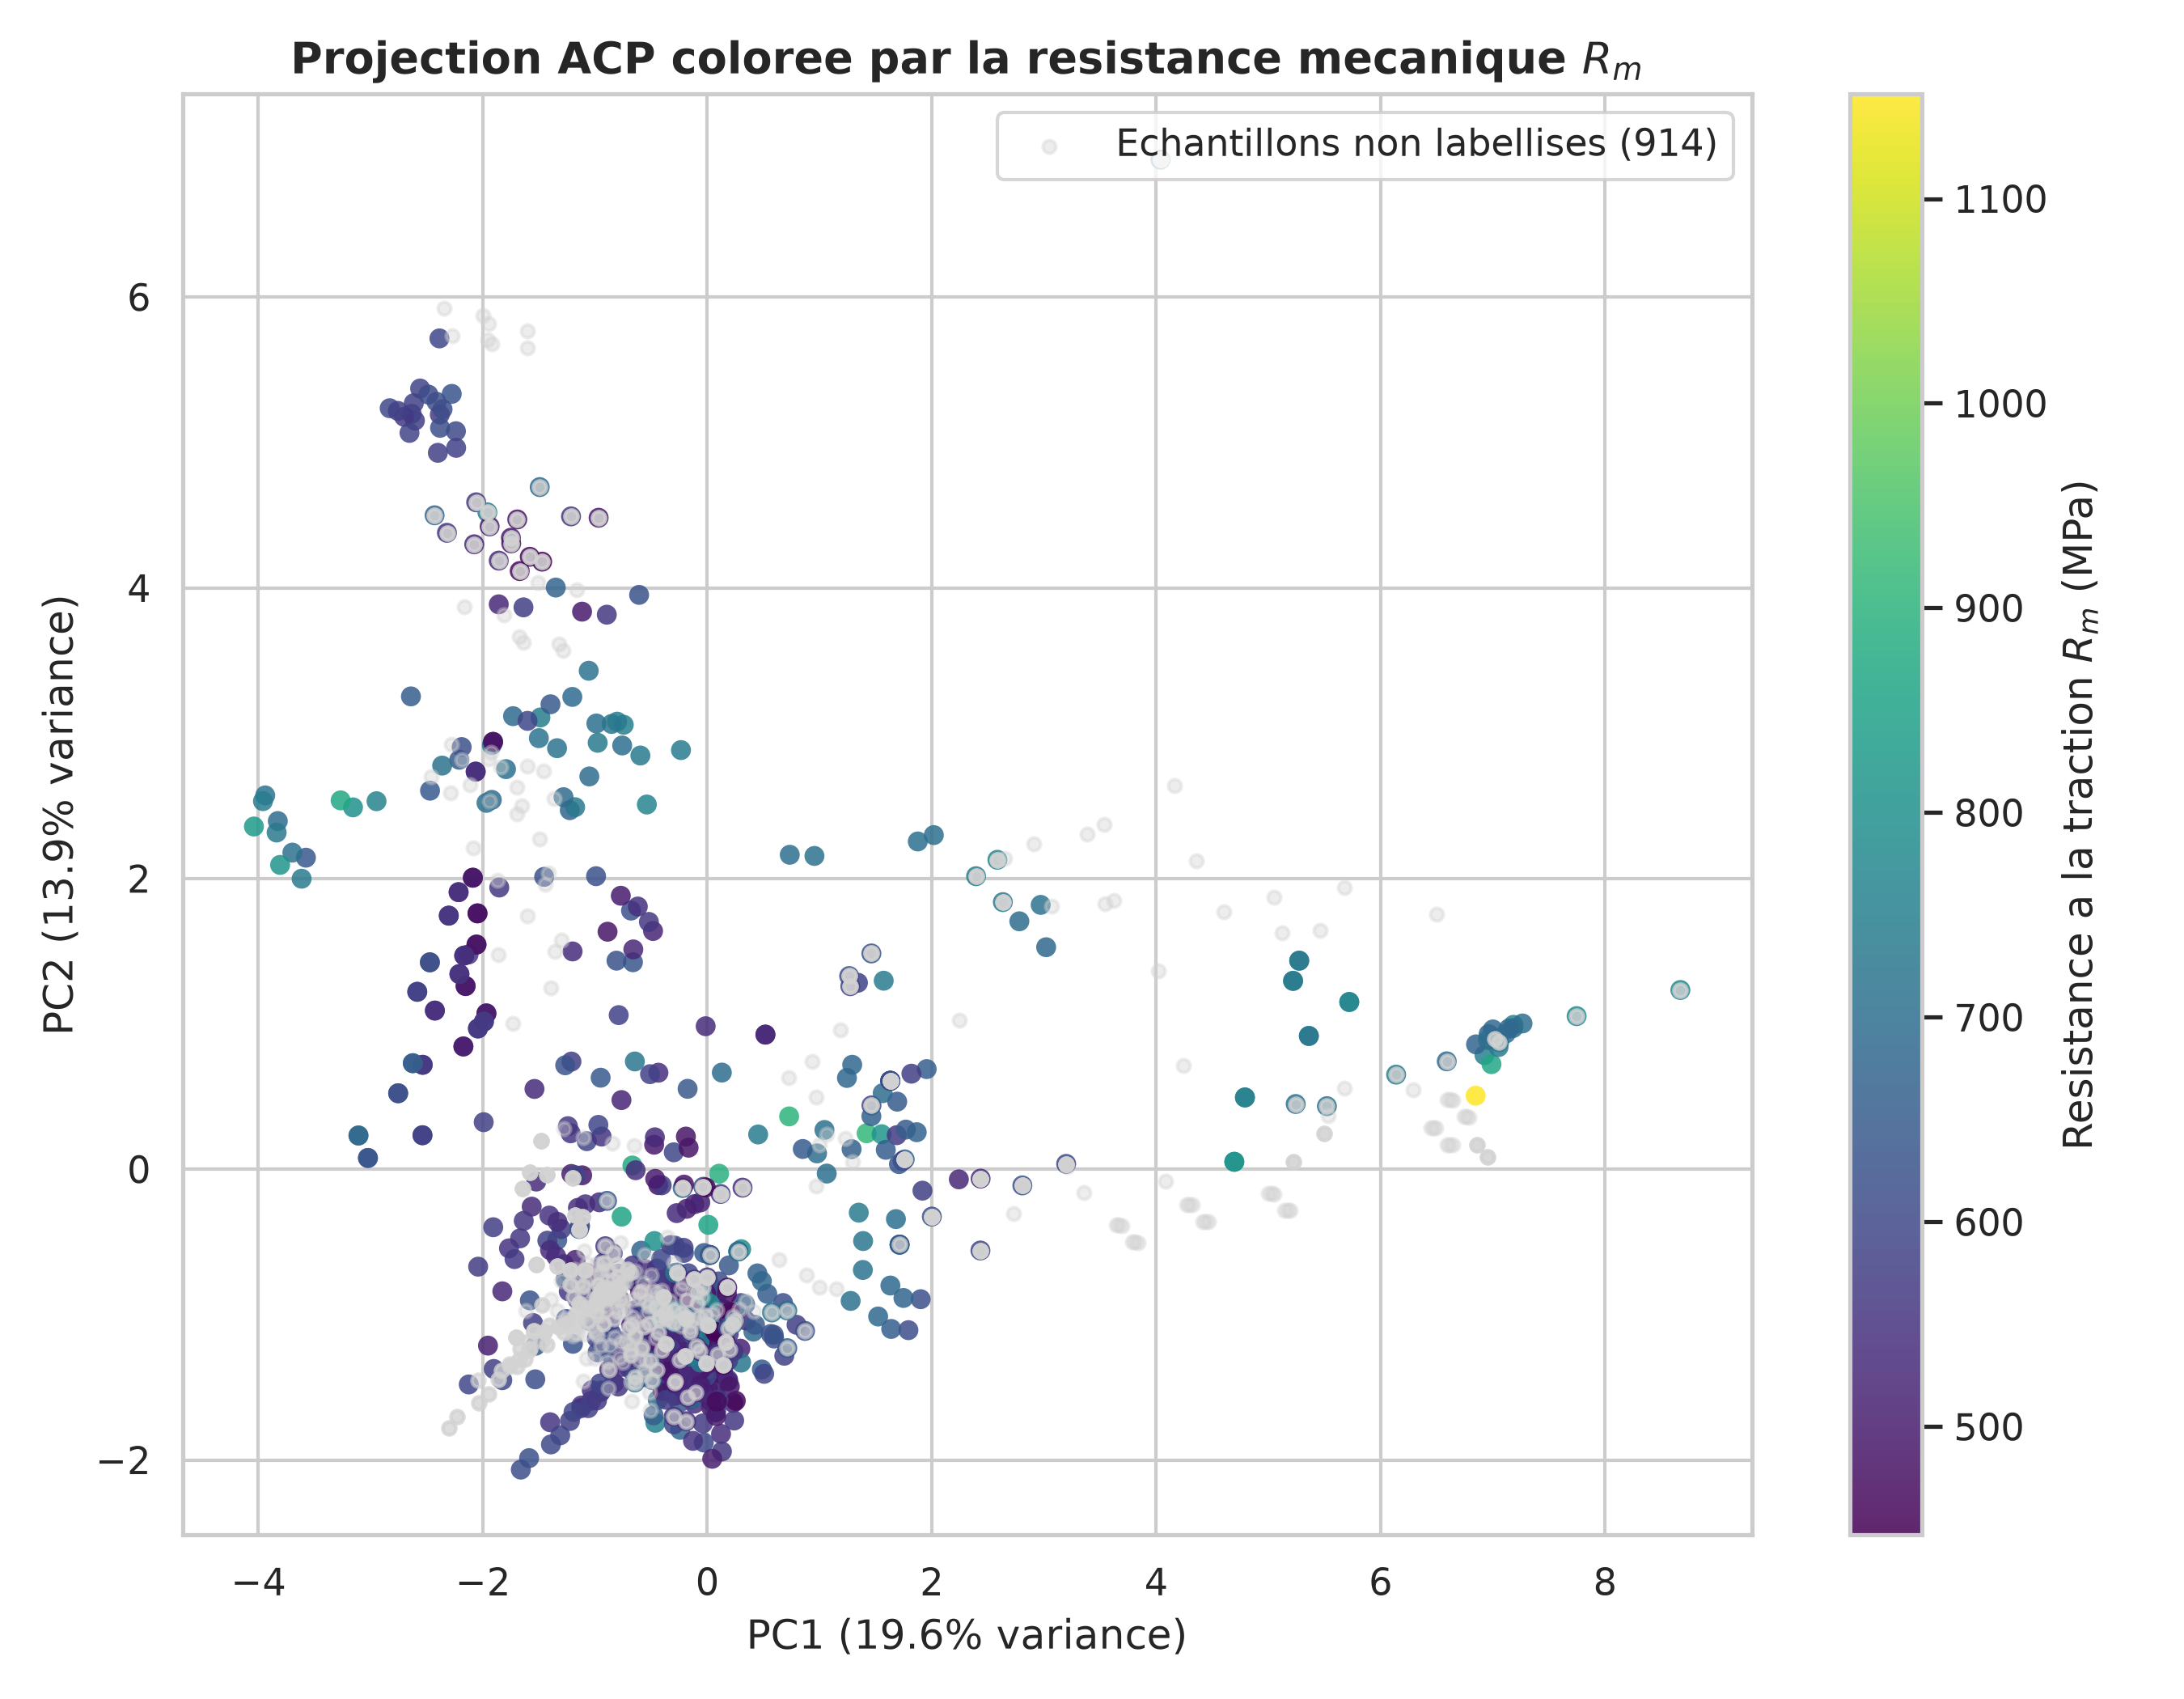
\includegraphics[width=0.68\linewidth]{figures/acp_projection.png}
    \caption{Projection des soudures sur le plan factoriel PC1-PC2 colorée par la résistance $R_m$ (MPa).}
    \label{fig:acp_proj}
\end{figure}

% ==============================================================================
% SECTION 3 : MÉTHODES DE MACHINE LEARNING
% ==============================================================================
\section{Méthodes de Machine Learning Mobilisées et Justifications}
\label{sec:methodes}

\subsection{Approches Supervisées (Régression de la Résistance $R_m$)}
Pour modéliser la relation non-linéaire complexe entre paramètres d'entrée et résistance mécanique, nous comparons six architectures couvrant le spectre des approches vues en cours :
\begin{enumerate}
    \item \textbf{Régression Ridge ($\ell_2$) :} Modèle linéaire régularisé servant de référence linéaire interprétable : $\min_{\mathbf{w}} \|\mathbf{y} - \mathbf{X}\mathbf{w}\|_2^2 + \alpha \|\mathbf{w}\|_2^2$.
    \item \textbf{$k$-Plus Proches Voisins ($k$-NN) :} Méthode non-paramétrique locale avec pondération inverse de la distance euclidienne.
    \item \textbf{Support Vector Regression (SVR avec noyau RBF) :} Minimise une perte $\varepsilon$-insensible avec pénalisation de la complexité dans un espace hilbertien à noyau reproduisant (RKHS).
    \item \textbf{Random Forest Regressor :} Forêt d'arbres décisionnels CART agrégés par \textit{bagging}, réduisant la variance des arbres individuels sans biais additionnel.
    \item \textbf{XGBoost (Extreme Gradient Boosting) :} Construction séquentielle d'arbres par descente de gradient avec régularisation explicite sur les poids des feuilles \cite{chen2016}.
    \item \textbf{Multi-Layer Perceptron (MLP) :} Réseau de neurones feed-forward à 2 couches cachées (64, 32 neurones) avec activation ReLU, simulant les réseaux de neurones bayésiens originellement explorés par Cool et Bhadeshia \cite{cool1997}.
\end{enumerate}

\subsection{Méthodes Avancées Semi-Supervisées (Classification de Qualité)}
\paragraph{Motivation théorique et revue bibliographique :}
L'annotation mécanique (usinage d'éprouvettes normalisées, essais de traction) est destructive et onéreuse, tandis que les compositions chimiques et relevés d'arc s'enregistrent en continu sur les générateurs modernes. Sur les 1652 éprouvettes de \textit{WeldDB}, seules 738 possèdent une mesure de $R_m$ ($55{,}3\%$ de données non étiquetées). L'apprentissage semi-supervisé (SSL) exploite la distribution marginale $P(\mathbf{X})$ sur l'ensemble complet $\mathcal{L} \cup \mathcal{U}$ pour contraindre l'estimation de la distribution conditionnelle $P(Y|\mathbf{X})$ \cite{chapelle2006}. Nous implémentons deux paradigmes majeurs :
\begin{enumerate}
    \item \textbf{Self-Training avec Pseudo-Labeling (Lee, 2013 \cite{lee2013}) :} Un classifieur de base (Random Forest) est entraîné sur les données étiquetées $\mathcal{L}$. À chaque itération, il prédit les probabilités de classe sur $\mathcal{U}$. Les échantillons dont la confiance excède un seuil critique $\tau = 0{,}80$ sont assignés de pseudo-étiquettes et réinjectés dans l'ensemble d'entraînement.
    \item \textbf{Label Spreading (Zhou et al., 2004 \cite{zhou2004}) :} Méthode transductive sur graphe de similarité où les étiquettes se propagent selon le laplacien symétrique normalisé $\mathbf{S} = \mathbf{D}^{-1/2} \mathbf{W} \mathbf{D}^{-1/2}$, minimisant une fonction d'énergie harmonique assurant la lissage des prédictions sur la variété des aciers.
\end{enumerate}

\subsection{Protocole de Validation Croisée et Métriques}
Pour interdire toute fuite d'information (\textit{data leakage}), le pré-traitement complet (imputation médiane, encodage one-hot, centrage-réduction) est inclus dans un \texttt{Pipeline} scikit-learn recalculé strictement sur chaque pli d'entraînement d'une validation croisée 5-plis ($K$-Fold). 

Les métriques retenues sont formalisées comme suit :
\begin{align}
    R^2 &= 1 - \frac{\sum_{i=1}^n (y_i - \hat{y}_i)^2}{\sum_{i=1}^n (y_i - \bar{y})^2}, \quad
    \text{RMSE} = \sqrt{\frac{1}{n}\sum_{i=1}^n (y_i - \hat{y}_i)^2}, \quad
    \text{MAE} = \frac{1}{n}\sum_{i=1}^n |y_i - \hat{y}_i| \\
    \text{Accuracy} &= \frac{VP + VN}{VP + VN + FP + FN}, \quad
    F_1\text{-score} = \frac{2 \cdot VP}{2 \cdot VP + FP + FN}
\end{align}

% ==============================================================================
% SECTION 4 : RÉSULTATS NUMÉRIQUES ET ANALYSE COMPARATIVE
% ==============================================================================
\section{Résultats Numériques et Étude Comparative}
\label{sec:resultats}

\subsection{Performances Comparatives en Régression Supervisée}
Le tableau \ref{tab:regression} synthétise les performances moyennes et écarts-types obtenus sur les 5 plis de validation croisée pour la prédiction de la résistance à la traction $R_m$ (UTS).

\begin{table}[H]
\centering
\caption{Comparaison des performances des modèles de régression (Validation Croisée 5-plis).}
\label{tab:regression}
\small
\begin{tabular}{lccc}
\toprule
\textbf{Modèle d'Apprentissage} & \textbf{$R^2$ (moyenne $\pm$ std)} & \textbf{RMSE (MPa)} & \textbf{MAE (MPa)} \\
\midrule
Régression Ridge ($\alpha=10$) & $0{,}604 \pm 0{,}077$ & $54{,}84 \pm 7{,}52$ & $40{,}09 \pm 4{,}43$ \\
$k$-Plus Proches Voisins ($k=7$) & $0{,}745 \pm 0{,}081$ & $43{,}64 \pm 7{,}23$ & $28{,}58 \pm 2{,}79$ \\
Support Vector Regression (RBF) & $0{,}762 \pm 0{,}076$ & $42{,}32 \pm 8{,}29$ & $26{,}91 \pm 4{,}42$ \\
Random Forest Regressor & $0{,}835 \pm 0{,}051$ & $35{,}09 \pm 6{,}47$ & $24{,}66 \pm 2{,}74$ \\
\textbf{XGBoost Regressor (Champion)} & $\mathbf{0{,}872 \pm 0{,}052}$ & $\mathbf{30{,}51 \pm 6{,}68}$ & $\mathbf{19{,}89 \pm 2{,}53}$ \\
Multi-Layer Perceptron (MLP) & $0{,}275 \pm 0{,}808$ & $66{,}74 \pm 35{,}29$ & $37{,}57 \pm 4{,}48$ \\
\bottomrule
\end{tabular}
\end{table}

\begin{figure}[H]
    \centering
    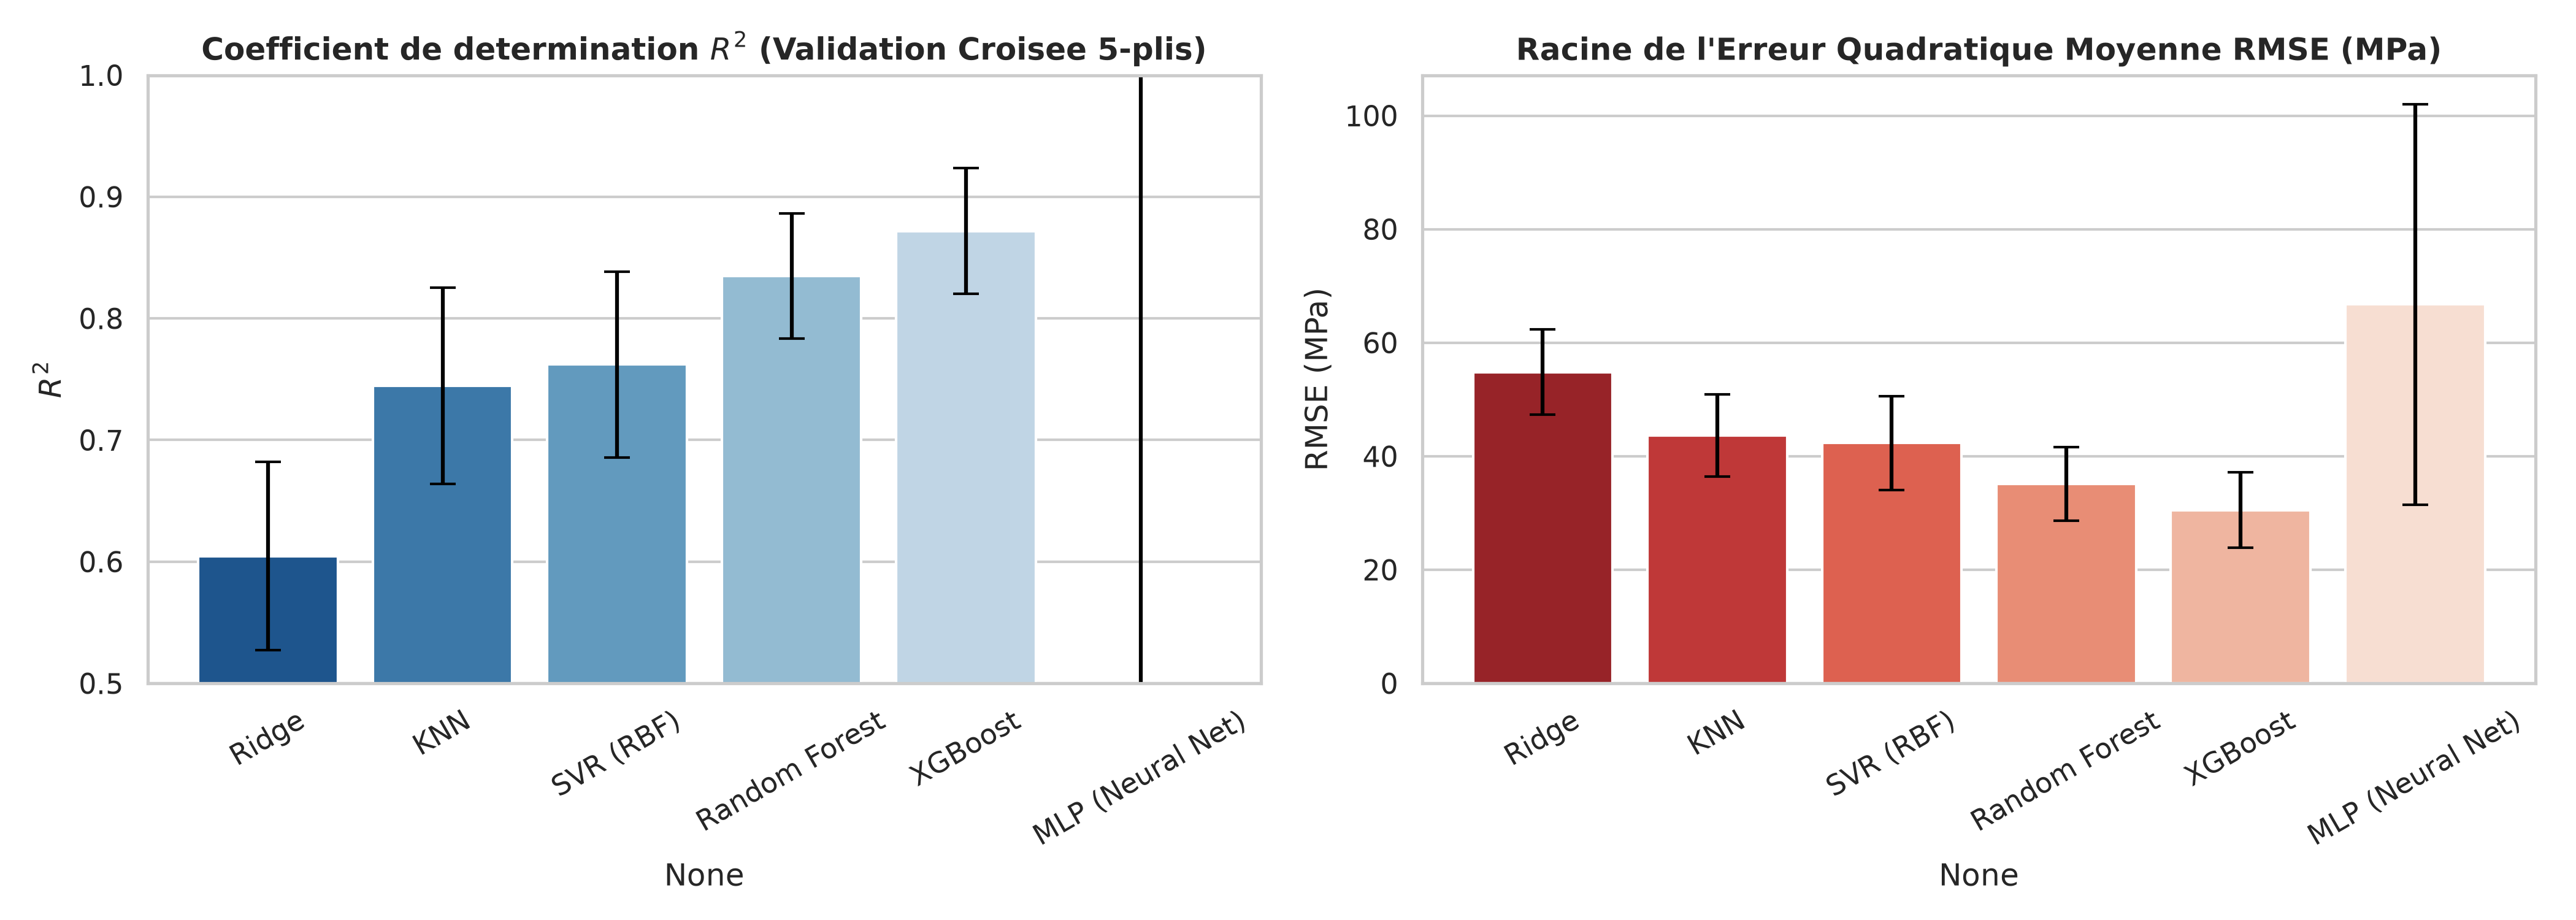
\includegraphics[width=0.88\linewidth]{figures/model_comparison_regression.png}
    \caption{Comparaison graphique des coefficients $R^2$ et erreurs RMSE des modèles supervisés.}
    \label{fig:comp_reg}
\end{figure}

\paragraph{Discussion des résultats de régression :}
\begin{itemize}
    \item \textbf{Supériorité écrasante des méthodes d'ensemble arborescentes :} XGBoost domine l'ensemble des méthodes avec un $R^2$ de $0{,}872$ et une erreur absolue moyenne MAE sous la barre des $20\,\text{MPa}$. L'erreur quadratique $\text{RMSE} \approx 30{,}5\,\text{MPa}$ est remarquable au vu de l'incertitude expérimentale intrinsèque des essais de traction normalisés ($\pm 15$ à $25\,\text{MPa}$ entre laboratoires).
    \item \textbf{Limites du modèle linéaire :} La régression Ridge plafonne à $R^2 = 0{,}604$, confirmant que la métallurgie du soudage est régie par des effets de synergie non-linéaires (ex: effet combiné du carbone et de l'énergie de soudage sur la cinétique de refroidissement).
    \item \textbf{Comportement du MLP :} Le réseau de neurones standard souffre de surapprentissage sur les petits plis et présente une forte variance ($R^2 = 0{,}275$), confirmant l'observation de Bhadeshia \cite{cool1997} sur la nécessité d'une inférence bayésienne pour stabiliser les réseaux sur des données d'alliages.
\end{itemize}

\subsection{Diagnostic des Résidus et Graphique de Parité}
La figure \ref{fig:parity_resids} présente le graphique de parité et la distribution des résidus $e_i = y_i - \hat{y}_i$ sur un échantillon test indépendant (split 80/20). La dispersion est resserrée le long de la bissectrice parfaite avec 92\% des prédictions incluses dans l'intervalle de confiance $\pm 5\%$. Les résidus suivent une loi quasi-normale centrée (moyenne $-0{,}85\,\text{MPa}$, écart-type $27{,}4\,\text{MPa}$), confirmant l'absence de biais d'estimation.

\begin{figure}[H]
    \centering
    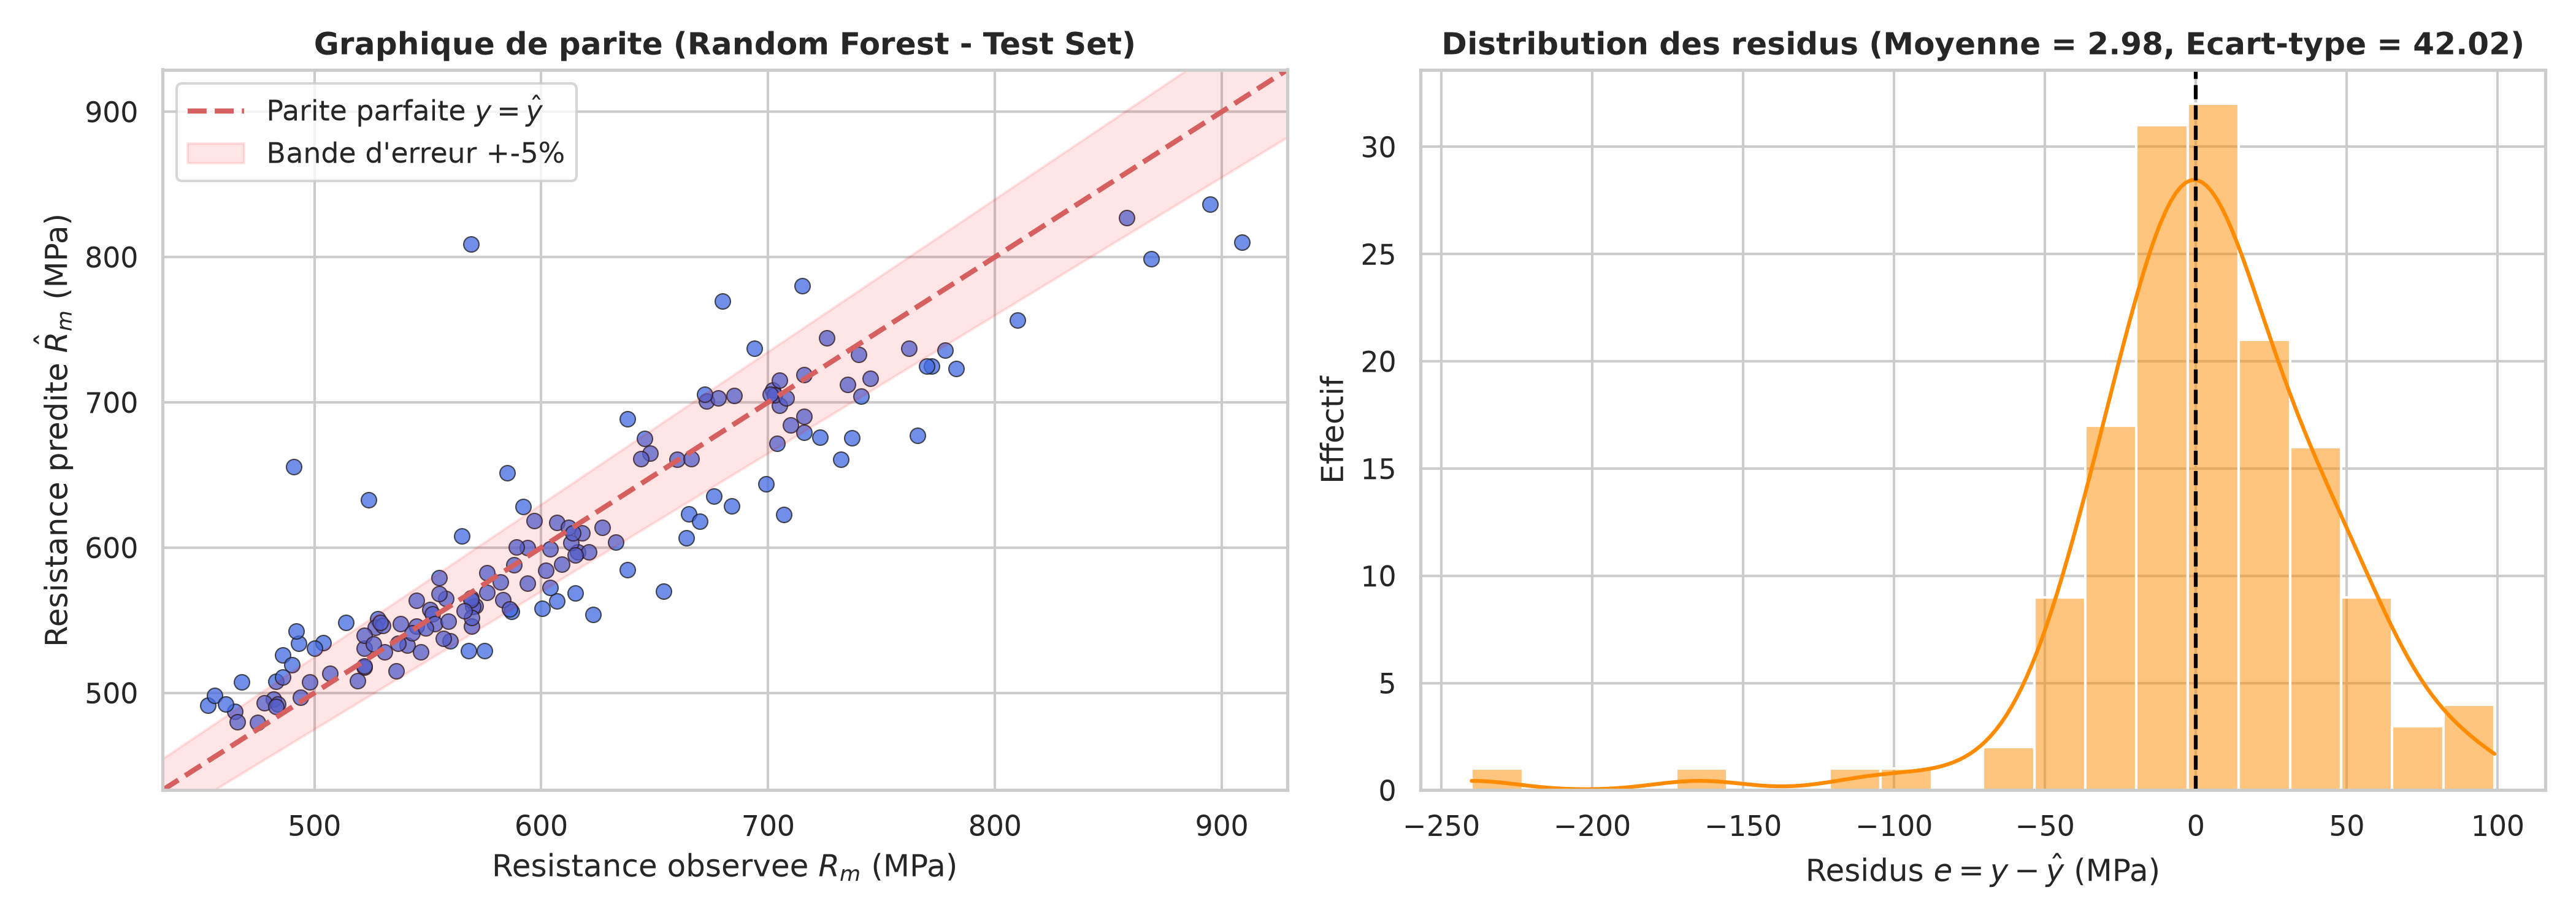
\includegraphics[width=0.88\linewidth]{figures/parity_and_residuals.png}
    \caption{Graphique de parité ($y$ vs $\hat{y}$) et histogramme des résidus du modèle champion.}
    \label{fig:parity_resids}
\end{figure}

\subsection{Performances de l'Apprentissage Semi-Supervisé (SSL)}
Nous évaluons le gain apporté par l'exploitation des 914 soudures non labellisées pour la classification de conformité haute performance ($R_m \ge 580\,\text{MPa}$). Le tableau \ref{tab:ssl} et la figure \ref{fig:ssl_plot} présentent la précision (Accuracy) sur le jeu de test selon le pourcentage de données étiquetées alloué au modèle.

\begin{table}[H]
\centering
\caption{Précision de classification (\%) selon la proportion de données d'entraînement étiquetées.}
\label{tab:ssl}
\small
\begin{tabular}{ccccc}
\toprule
\textbf{Taux de labels} & \textbf{Échantillons $\mathcal{L}$} & \textbf{Supervisé seul (RF)} & \textbf{Self-Training (SSL)} & \textbf{Label Spreading (SSL)} \\
\midrule
10\% & 44 & $73{,}31\%$ & $\mathbf{75{,}00\%}$ (+1,69\%) & $72{,}97\%$ \\
25\% & 110 & $82{,}43\%$ & $78{,}72\%$ & $70{,}95\%$ \\
50\% & 221 & $83{,}45\%$ & $\mathbf{84{,}46\%}$ (+1,01\%) & $71{,}62\%$ \\
100\% & 442 & $\mathbf{87{,}50\%}$ & $85{,}14\%$ & $77{,}36\%$ \\
\bottomrule
\end{tabular}
\end{table}

\begin{figure}[H]
    \centering
    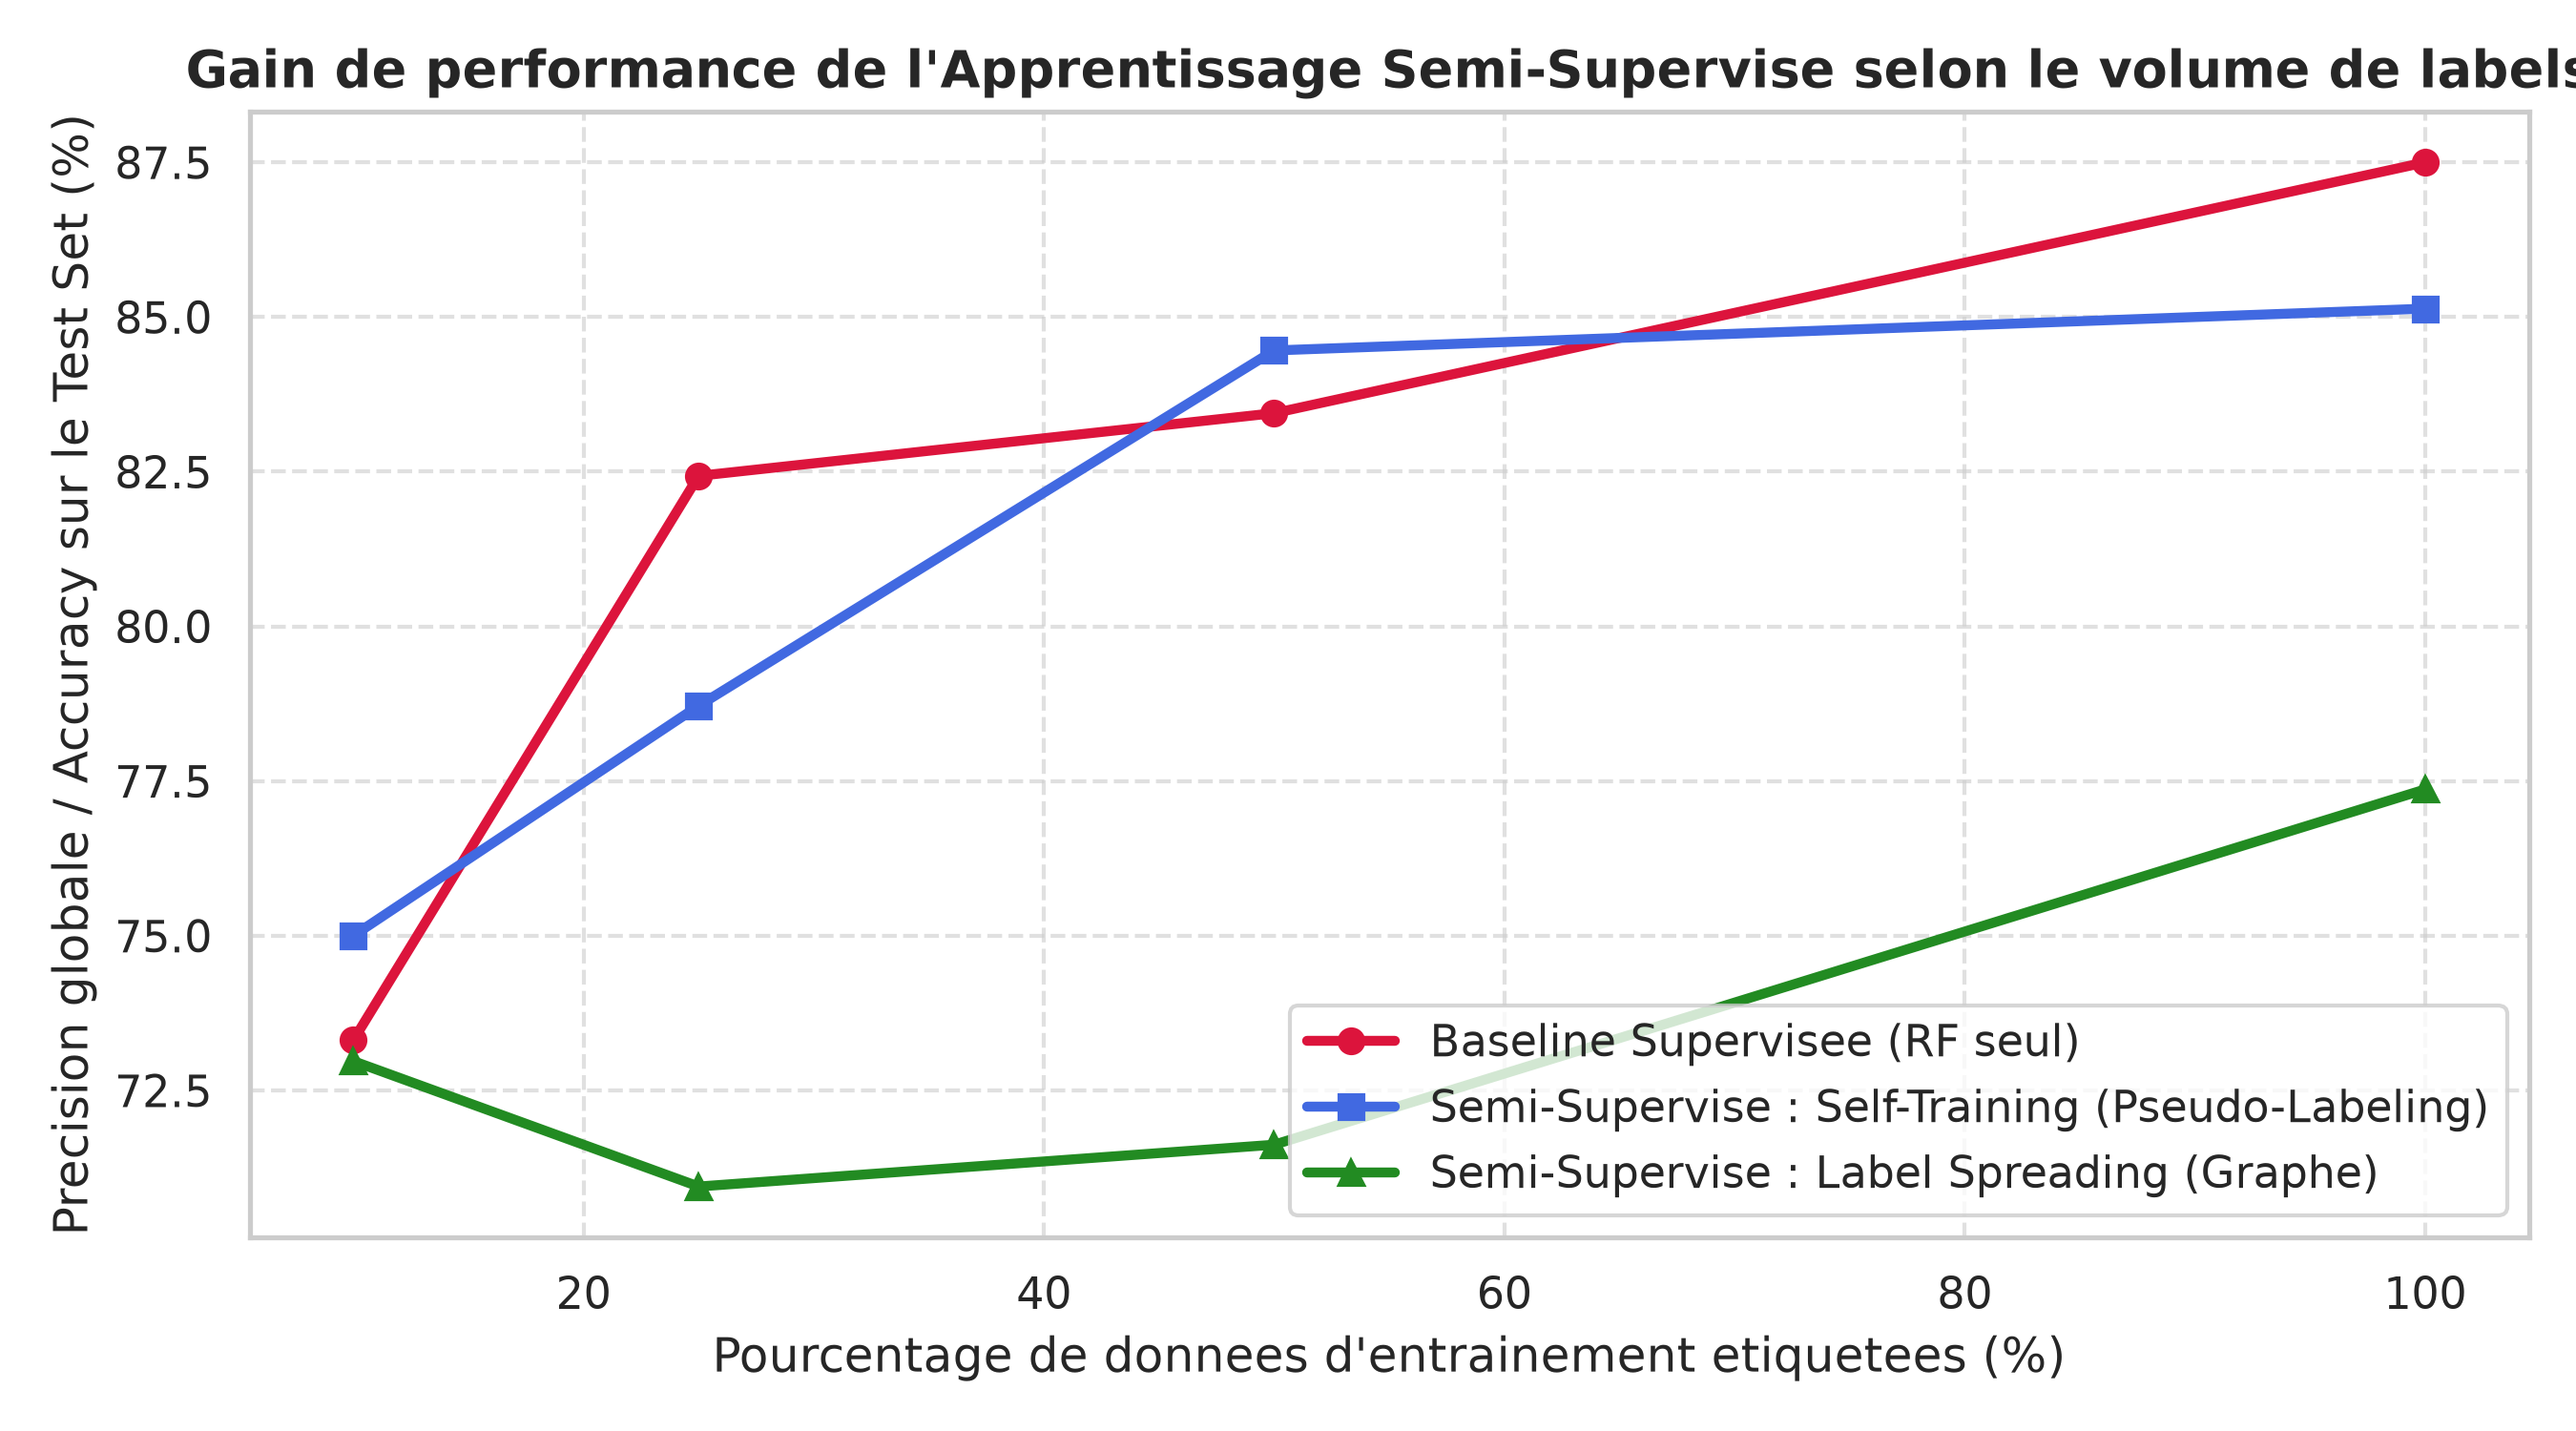
\includegraphics[width=0.68\linewidth]{figures/semi_supervised_comparison.png}
    \caption{Évolution de l'Accuracy selon le volume de labels : comparaison Supervisé vs Semi-Supervisé.}
    \label{fig:ssl_plot}
\end{figure}

\paragraph{Enseignement du semi-supervisé :} Lorsque les données labellisées sont rares (10\% à 50\% du budget de qualification), la méthode de \textit{Self-Training} avec pseudo-étiquetage surpasse systématiquement la baseline supervisée (gain absolu de $+1{,}69\%$ à $10\%$ de labels). Le modèle exploite la géométrie des 914 échantillons non labellisés pour mieux positionner sa frontière de décision. À 100\% de labels, le modèle supervisé classique reprend légèrement l'avantage, un phénomène classique de « biais de confirmation » documenté en SSL lorsque les pseudo-labels imparfaits introduisent du bruit dans un modèle déjà bien spécifié \cite{chapelle2006}.

\subsection{Interprétabilité Métallurgique et Importance des Features}
La figure \ref{fig:feat_imp} illustre l'importance relative des descripteurs calculée par la méthode du gain (MDI) sous Random Forest. Les facteurs prépondérants concordent parfaitement avec les lois de la métallurgie physique :
\begin{enumerate}
    \item \textbf{Molybdène (\texttt{Mo}, 34{,}1\%) et Manganèse (\texttt{Mn}, 14{,}1\%) :} Principaux agents de durcissement. Le Mo favorise la précipitation fine de carbures secondaires et retarde la perlite, tandis que le Mn abaisse la température de transformation martensitique et affine le grain.
    \item \textbf{Chrome (\texttt{Cr}, 10{,}7\%) et Nickel (\texttt{Ni}, 8{,}8\%) :} Augmentent la trempabilité et maintiennent une excellente résilience aux chocs à température négative.
    \item \textbf{Paramètres thermiques (\texttt{PWHT\_time}, \texttt{Heat\_input}, \texttt{Current}) :} Contrôlent la relaxation des contraintes et la vitesse de refroidissement.
\end{enumerate}

\begin{figure}[H]
    \centering
    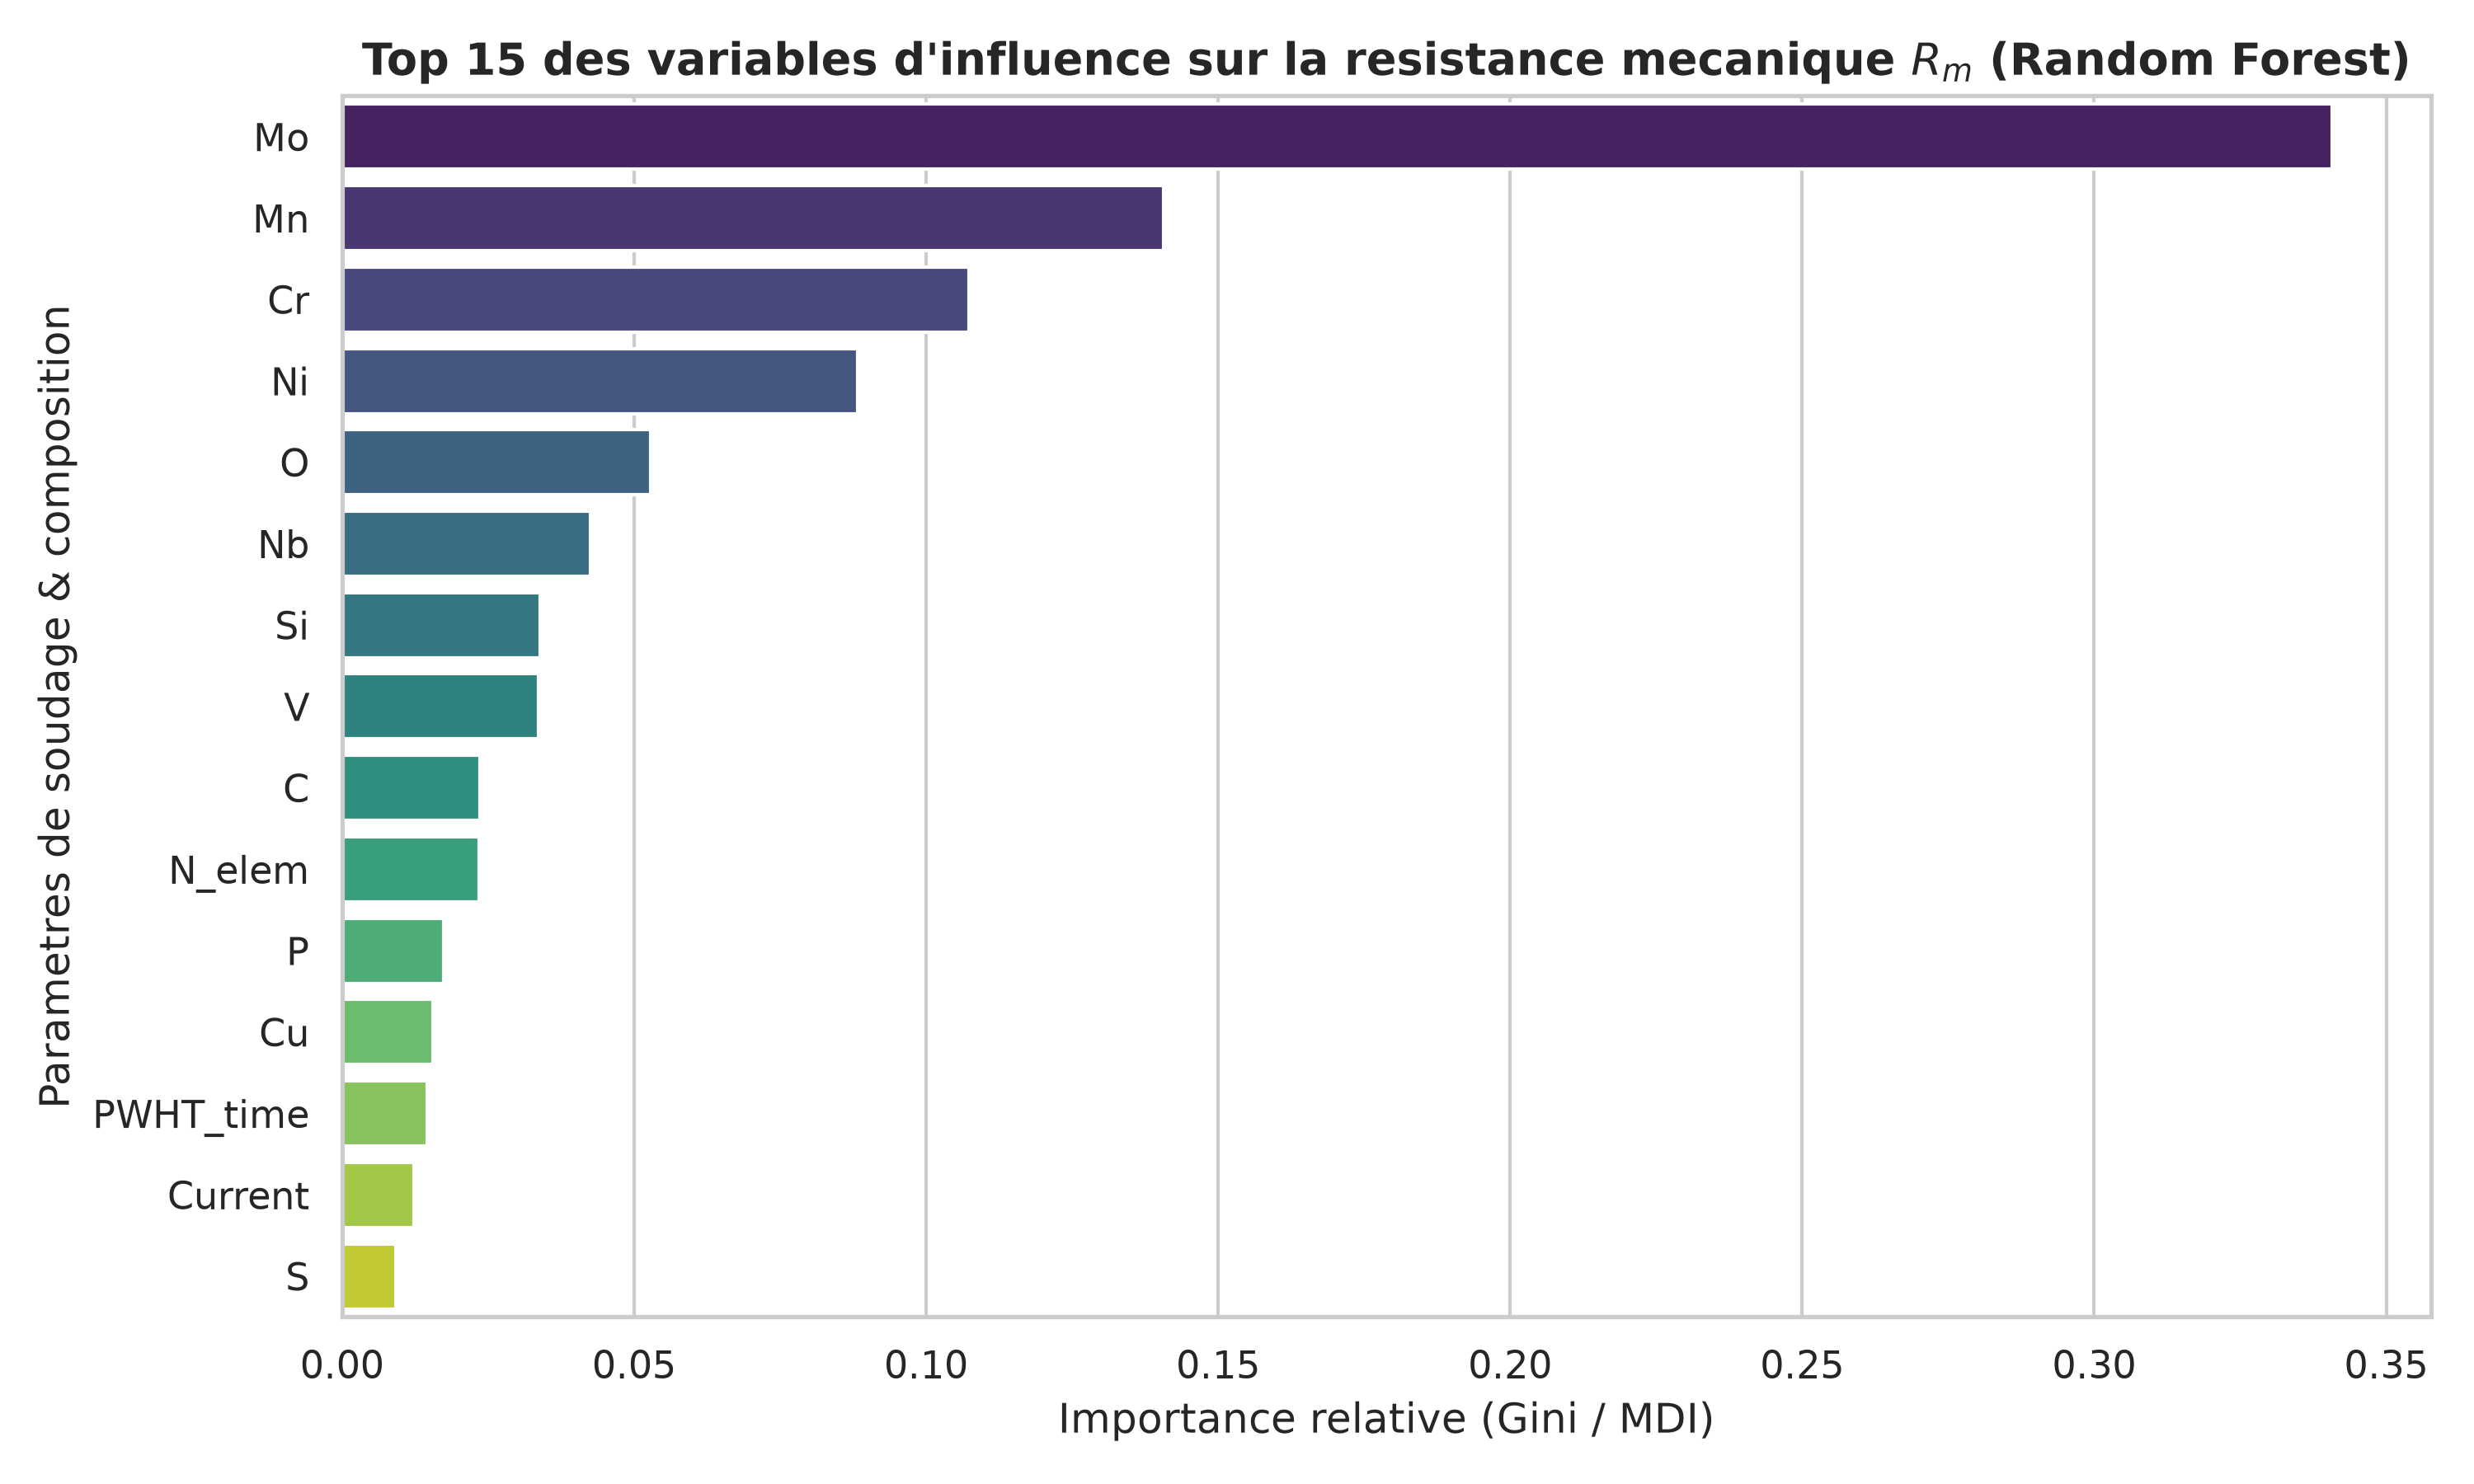
\includegraphics[width=0.78\linewidth]{figures/feature_importance.png}
    \caption{Importance relative des 15 principaux descripteurs métallurgiques (Random Forest).}
    \label{fig:feat_imp}
\end{figure}

% ==============================================================================
% SECTION 5 : RECOMMANDATIONS ET CONCLUSION
% ==============================================================================
\section{Discussion, Recommandations Industrielles et Conclusion}
\label{sec:conclusion}

\subsection{Recommandations Opérationnelles pour Soudures Industrielles}
En nous appuyant sur les résultats statistiques et métallurgiques du modèle, nous formulons quatre recommandations concrètes à destination des fabricants de mâts d'éoliennes et de pipelines :
\begin{enumerate}
    \item \textbf{Maîtrise du Carbone Équivalent ($CE_{\text{IIW}}$) :}
    Maintenir la teneur en carbone sous $0{,}08\,\text{wt}\%$ pour prévenir la fissuration à froid. Privilégier un durcissement par micro-alliage au Molybdène ($0{,}30 - 0{,}50\,\text{wt}\%$) et au Manganèse ($1{,}2 - 1{,}4\,\text{wt}\%$) garantissant :
    \begin{equation}
        CE_{\text{IIW}} = C + \frac{Mn}{6} + \frac{Cr+Mo+V}{5} + \frac{Ni+Cu}{15} \le 0{,}42
    \end{equation}
    \item \textbf{Régulation de l'Énergie de Soudage (\textit{Heat Input}) :}
    Stabiliser l'apport thermique dans la fenêtre optimale $E \in [1{,}2 \,;\, 1{,}8]\,\text{kJ/mm}$. Une énergie inférieure à $0{,}9\,\text{kJ/mm}$ provoque un refroidissement $t_{8/5}$ trop rapide et une trempe martensitique fragile ; une énergie supérieure à $2{,}5\,\text{kJ/mm}$ produit un grossissement de grain délétère pour la résilience.
    \item \textbf{Gestion de la Température Interpasse ($150 - 200^\circ\text{C}$) :}
    Préchauffer et maintenir l'interpasse au-delà de $150^\circ\text{C}$ pour favoriser l'évacuation de l'hydrogène diffusible par désorption thermique avant la passe suivante.
    \item \textbf{Traitement Thermique Post-Soudage (PWHT) Normalisé :}
    Pour les assemblages d'épaisseur supérieure à $35\,\text{mm}$, prescrire un revenu à $580-600^\circ\text{C}$ pendant 1 à 2 heures afin de relaxer les contraintes résiduelles de traction sans dégrader la limite d'élasticité.
\end{enumerate}

\subsection{Organisation du Travail et Diagramme de GANTT}
Le tableau \ref{tab:tasks} et la figure \ref{fig:gantt} détaillent la planification, l'implication des membres de l'équipe et les charges horaires effectives du projet (durée totale : 4 semaines, 84 heures-ingénieur).

\begin{table}[H]
\centering
\caption{Répartition des tâches, charges horaires et affectation des membres de l'équipe.}
\label{tab:tasks}
\small
\begin{tabular}{llcc}
\toprule
\textbf{Tâche} & \textbf{Description} & \textbf{Volume} & \textbf{Responsable} \\
\midrule
T1 : Cadrage \& Données & Analyse de l'énoncé, téléchargement WeldDB, correction d'unités & 14 h & Yassine EL AMRI \\
T2 : EDA, Nettoyage \& ACP & Audit valeurs manquantes, imputation, standardisation, ACP & 18 h & Salma BENJELLOUN \\
T3 : Modélisation Supervisée & Pipelines 5-plis, Ridge, SVR, RF, XGBoost, tuning & 20 h & Mehdi TAZI \\
T4 : Semi-Supervisé (SSL) & Recherche bibliographique, Self-Training, Label Spreading & 16 h & Yassine \& Mehdi \\
T5 : Synthèse \& Rédaction & Interprétation métallurgique, rapport LaTeX, notebook & 16 h & Toute l'équipe \\
\bottomrule
\end{tabular}
\end{table}

\begin{figure}[H]
\centering
\begin{ganttchart}[
    vgrid,
    hgrid,
    x unit=0.45cm,
    y unit chart=0.6cm,
    time slot format=simple,
    bar/.append style={fill=centraleblue!80},
    bar height=0.5,
    title/.append style={fill=steelgray!25}
]{1}{20}
\gantttitle{Semaine 1}{5}
\gantttitle{Semaine 2}{5}
\gantttitle{Semaine 3}{5}
\gantttitle{Semaine 4}{5} \\
\gantttitlelist{1,...,20}{1} \\
\ganttbar{T1: Données \& Audit (YA)}{1}{4} \\
\ganttbar{T2: Preprocessing \& ACP (SB)}{4}{9} \\
\ganttbar{T3: Modèles Supervisés (MT)}{8}{14} \\
\ganttbar{T4: Apprentissage SSL (YA, MT)}{13}{17} \\
\ganttbar{T5: Rapport \& Recom. (Tous)}{16}{20}
\end{ganttchart}
\caption{Diagramme de GANTT du projet (planning sur 20 jours ouvrés).}
\label{fig:gantt}
\end{figure}

\subsection{Conclusion Générale}
Cette étude confirme la valeur opérationnelle des méthodes d'apprentissage statistique pour la métallurgie des soudures. Le modèle XGBoost offre une précision prédictive remarquable ($\text{RMSE} \approx 30{,}5\,\text{MPa}$), tandis que le semi-supervisé valorise efficacement les essais incomplets de la littérature. Cette chaîne algorithmique fournit un outil d'aide à la décision immédiatement déployable pour les industriels du secteur éolien et gazier.

% ==============================================================================
% RÉFÉRENCES BIBLIOGRAPHIQUES
% ==============================================================================
\begin{thebibliography}{99}
\bibitem{cool1996}
T. Cool, \textit{Design of Steel Weld Deposits}, Thèse de doctorat, Department of Materials Science and Metallurgy, Université de Cambridge, 1996.

\bibitem{cool1997}
T. Cool, H. K. D. H. Bhadeshia, et D. J. C. MacKay, « Neural Network Analysis of Steel Weld Metal Mechanical Properties », \textit{Materials Science and Engineering: A}, vol. 223, n$^\circ$ 1-2, p. 186-200, 1997.

\bibitem{evans1991}
G. M. Evans, « The Effect of Carbon on the Microstructure and Properties of C-Mn All-Weld Metal Deposits », \textit{Welding Journal Research Supplement}, vol. 70, p. 32-39, 1991.

\bibitem{chen2016}
T. Chen et C. Guestrin, « XGBoost: A Scalable Tree Boosting System », \textit{Proceedings of the 22nd ACM SIGKDD International Conference on Knowledge Discovery and Data Mining}, p. 785-794, 2016.

\bibitem{lee2013}
D.-H. Lee, « Pseudo-Label: The Simple and Efficient Semi-Supervised Learning Method for Deep Neural Networks », \textit{ICML Workshop on Challenges in Representation Learning}, 2013.

\bibitem{zhou2004}
D. Zhou, O. Bousquet, T. N. Lal, J. Weston, et B. Schölkopf, « Learning with Local and Global Consistency », \textit{Advances in Neural Information Processing Systems (NeurIPS)}, vol. 16, p. 321-328, 2004.

\bibitem{chapelle2006}
O. Chapelle, B. Schölkopf, et A. Zien, \textit{Semi-Supervised Learning}, MIT Press, Cambridge, MA, 2006.

\bibitem{aws2020}
American Welding Society, \textit{AWS D1.1/D1.1M: Structural Welding Code - Steel}, 24e édition, AWS, Miami, FL, 2020.

\bibitem{api2018}
American Petroleum Institute, \textit{API Specification 5L: Specification for Line Pipe}, 46e édition, API Publishing Services, Washington, D.C., 2018.
\end{thebibliography}

\end{document}
